\chapter{Modulation}
\label{Modulation}


\begin{center}
\begin{figure}[h!]
\tikzset{concept/.append style={fill={none}}}
\begin{tikzpicture}
  \path[mindmap,concept color=black,text=black]
    node[concept] {Modulation}
    [clockwise from=0]
    child[concept color=green!50!black] {
      node[concept] {AM}
      % }
      [clockwise from=90]
      child { node[concept] {AM} }
      child { node[concept] {Ring Modulation} }
      % child { node[concept] {pro\-gramming languages} }
      % child { node[concept] {software engineer\-ing} }
    }  
    child[concept color=blue] {
      node[concept] (fm) {FM} 
      [clockwise from=-30]
    }
    child[concept color=red] { node[concept] (pm){Phase Modulation} }
    child[concept color=orange] { node[concept] (sd) {Sound design Challenge} };


\begin{pgfonlayer}{background}
    \draw [circle connection bar]
      (fm) edge (sd)
      (fm) edge (pm);
  \end{pgfonlayer}

\end{tikzpicture}
\caption{Lecture Contents}
\end{figure}
\end{center}


\section{Notizen}

kürzer. Modulation als sub einheit einplanen.
Sounddesign challg. halbe stunde ok..

Passt garnicht: (weil eher additive synth)
https://www.youtube.com/watch?v=oKv9S6mxnXE


Notation durchgehen.

Aliasing besprochen?
\href{https://www.youtube.com/watch?v=GBtHeR-hY9Y}{Water experiment}
(youtube \glqq{}The Secret to Levitation\grqq{})

AM, tremolo

Envelopes in pd

FM, vibrato

sounddesign chall.

Hü




\section{AM} % (fold)
\label{sub:AM}

Amplitude Modulation. \glqq{}tremolo\grqq{}


\begin{figure}[H]
	\begin{center}
		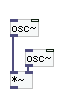
\includegraphics[width = 4cm]{img/ringNaive.png}
		\caption{naive Ring modulation}
		\label{fig:name}
	\end{center}
\end{figure}


\begin{figure}[H]
	\begin{center}
		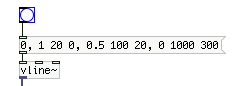
\includegraphics[width = 14cm]{img/simpleEnv.png}
		\caption{caption}
		\label{fig:name}
	\end{center}
\end{figure}

\textbf{Multiplying two signals in the time domain is equvalent to convolution in the frequency domain and vice versa.
}

Ringmodulation = Bipolar,
AM = Unipolar

\section{FM} % (fold)
\label{sub:FM}

Frequency Modulation. \glqq{}Vibrato\grqq{}


\begin{figure}[H]
	\begin{center}
		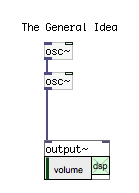
\includegraphics[width = 7cm]{img/FMgeneral.png}
		\caption{The General Idea of FM}
		\label{fig:fmIdea}
	\end{center}
\end{figure}

Naive parameters are ${f_c}$ (Carrier Frequency), ${f_m}$ (Modulator Frequency), and ${A_m}$ (modulation Amount).

\begin{figure}[H]
	\begin{center}
		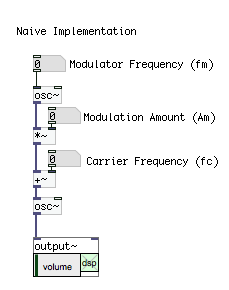
\includegraphics[width = 10cm]{img/FMnaive.png}
		\caption{Naive Implementation with Direct Parametrization.}
		\label{fig:fmNaive}
	\end{center}
\end{figure}

The output frequencies will be
\begin{equation}
	f_c \pm n \cdot f_m
\end{equation}

Typically, FM is controlled via \textit{Index}, \textit{Ratio}, and fundamental Frequency. The Index, ${I}$ is given by Modulation Depth and Modulator Frequency.

\begin{equation}
I = \frac{A_m}{f_m}
\end{equation}

A more controllable Implementation will generate the naive parameters from a Ratio, ${R}$, the Carrier Frequency and the Index:
\begin{equation}
	f_m = \frac{f_c}{R}
\end{equation}

\begin{equation}
	A_m = \frac{I}{f_m}
\end{equation}

\begin{figure}[H]
	\begin{center}
		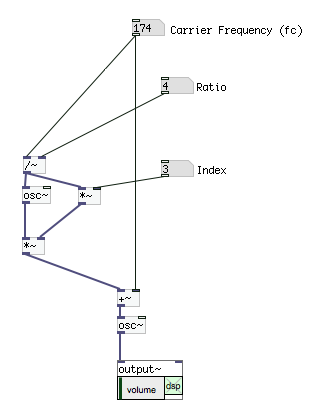
\includegraphics[width = 14cm]{img/FMcorrect.png}
		\caption{FM with Index and Ratio}
		\label{fig:fmComplete}
	\end{center}
\end{figure}

\section{Hausübung}
\label{sub:Hausuebung}
Andy Farnell, \href{http://aspress.co.uk/ds/pdf/pd_intro.pdf}{pd intro} chapter 6, lesen
